\documentclass[../Cours.tex]{subfiles}
\begin{document}

\chapitre{Divisibilité et nombres premiers}
\partie{Multiples et diviseurs}
\souspartie{Division euclidienne}

\definition{Soient deux nombres entiers $n$ et $p$. Il existe deux nombres $q$ et $r$ tels que : $$n = p \times q + r ~~~~~~(\mbox{avec}~~ 0 \infeg r < q)$$}

\exemple{%
\begin{center}
    \begin{tikzpicture}[scale=0.7]
        \node[anchor=south west] at (0,0) {
            \begin{tabularx}{0.17\textwidth}{CCC|CC}
                  & 6 & 5 & 4 &   \\
                - & 4 &   & 1 & 6 \\
                  & 2 & 5 &   &   \\
                - & 2 & 4 &   &   \\
                  &   & 1 &   &   \\
            \end{tabularx}
        };
        \draw (0.5,3) -- (2,3);
        \draw (0.5,1.1) -- (2.89,1.1);
        \draw (2.89,3.8) -- (4,3.8);
        \draw[noir,-Latex] (-2,4.2) -- (1,4.2); 
        \draw[noir,-Latex] (7,4.2) -- (4,4.2);
        \draw[noir,-Latex] (-2,0.7) -- (2,0.7);
        \draw[noir,-Latex] (7,3.4) -- (4.8,3.4);
        \node[anchor=east] at (-2,0.7) {\color{noir} Reste};
        \node[anchor=east] at (-2,4.2) {\color{noir} Dividende};
        \node[anchor=west] at (7,4.2) {\color{noir} Diviseur};
        \node[anchor=west] at (7,3.4) {\color{noir} Quotient};
        \node at (2.8,-2) {\Large{\color{rouge} \fbox{$65 = 4 \times 16 + 1$}}};
    \end{tikzpicture}
\end{center}
}

\souspartie{Critère de divisibilité}

\definition{On dit qu'un nombre $n$ est divisible par $q$ si le reste de la division euclidienne $n\div q$ vaut 0.}

\begin{listedexemples}
    \item $42$ est divisible par \textcolor{rouge}{6} car $42 = \textcolor{rouge}{6} \times 7$.
    \item $35$ est divisible par \textcolor{rouge}{5} car $35 = \textcolor{rouge}{5} \times 7$.
\end{listedexemples}

\paragraphe{noir}{Critères de divisibilité}{
    \begin{tabularx}{\textwidth}{l|C|l}
        & règle & exemples \\\hline
        divisible par 2 & \makecell{le nombre est pair \\ le chiffre des unités est 0, 2, 4, 6 ou 8} & \makecell{\textcolor{vert}{102 est pair}\\ \textcolor{rouge}{113 est impair}} \\\hline
        divisible par 5 & le chiffre des unités est 0 ou 5 & \makecell{\textcolor{vert}{\num{1000000005}} \\ \textcolor{rouge}{22} } \\\hline
        divisible par 10 & le chiffre des unités est 0 & \makecell{ \textcolor{vert}{\num{4000000000}} \\ \textcolor{rouge}{13} } \\\hline
        divisible par 3 & la somme des chiffres est dans la table de 3 & \makecell{\textcolor{vert}{213 $\longrightarrow 2+1+3 = 6$}\\\textcolor{rouge}{$17 \longrightarrow 1+7 = 8$}} \\\hline
        divisible par 9 & la somme des chiffres est dans la table de 9 & \makecell{\textcolor{vert}{342 $\longrightarrow 3+4+2 = 9$}\\\textcolor{rouge}{$14 \longrightarrow 1+4 = 5$}} \\\hline
    \end{tabularx}
}

\partie{Nombres premiers}
\souspartie{Concept}

\definition{Un nombre premier est un nombre entier ($\neq 1$) pour lequel les seuls diviseurs sont $1$ et lui-même.}

\paragraphe{noir}{Liste des nombres premiers $\infeg 30$}{2 ; 3 ; 5 ; 7 ; 11 ; 13 ; 17 ; 19 ; 23 ; 29}

\begin{listedexemples}
    \item 7 est un nombre premier car ses seuls diviseurs sont 1 et 7.
    \item 6 n'est pas un nombre premier car 2 et 3 sont des diviseurs de 6. \\ En effet, $6 = 2 \times 3$.
\end{listedexemples}

\souspartie{Décomposition en facteurs premiers}
\theoreme{\textsc{fondamental de l'arithmétique}}{Tout nombre entier peut se décomposer de manière unique (à l'ordre des facteurs près) en un produit de nombres premiers.}

\begin{listedexemples}
    \item $35 = 5 \times 7$
    \item $216 = 2 \times 2 \times 2 \times 3 \times 3 \times 3 $
\end{listedexemples}

\souspartie{Application : simplification de fraction}

\methode{Pour simplifier le plus possible une fraction, on peut décomposer en facteurs premiers le numérateur et le dénominateur.}

\renewcommand{\CancelColor}{\color{rouge}}
\renewcommand{\labelitemii}{$\blacksquare$}
\begin{listedexemples}
\item Pour simplifier la fraction $\dfrac{39}{65}$ :
\begin{itemize}
\item Je décompose le numérateur : $39=3 \times 13$
\item Je décompose le dénominateur : $65=5 \times 13$
\item Donc $\dfrac{39}{65} = \dfrac{3 \times 13}{5 \times 13} = \dfrac{3 \times \cancel{13}}{5 \times \cancel{13}} = \dfrac{3}{5}$
\end{itemize}
\end{listedexemples}

\souspartie{Primalité}

\theoreme{d'Euclide sur les nombres premiers}{
    Il existe une infinité de nombres premiers.
}

\paragraphe{noir}{Test de primalité \emph{simple} (Comment vérifier qu'un nombre est premier ?)}{
Pour vérifier qu'un nombre est premier, il faut vérifier qu'aucun nombre entier plus petit que lui (à part 1) n'est pas un de ses diviseurs.
}

\exemple{Vérifions que 7 est un nombre premier :
\begin{itemize}
    \foreach \n in {2,...,6}{
        \item 7 n'est pas divisible par \n{} car $7 \div \n$ n'est pas un entier
    }
\end{itemize}}

\clearpage
\begin{questions}
    \exercice Compléter le tableau suivant
    
    \begin{center}
    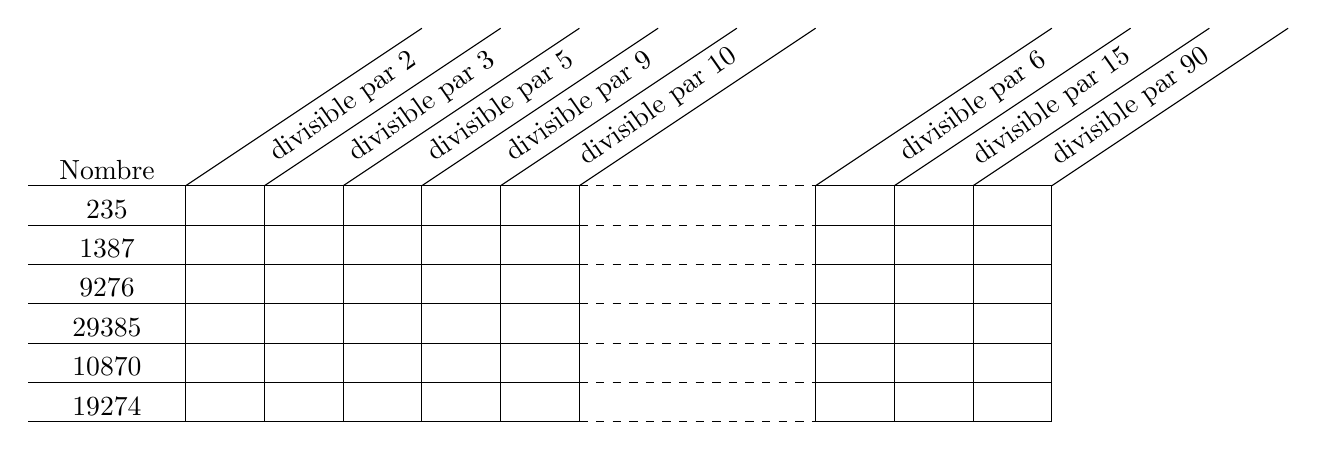
\begin{tikzpicture}
        \node at (1,0.2) {Nombre};
        \node at (1,-0.3) {235};
        \node at (1,-0.8) {1387};
        \node at (1,-1.3) {9276};
        \node at (1,-1.8) {29385};
        \node at (1,-2.3) {10870};
        \node at (1,-2.8) {19274};
        \foreach \y in {0,0.5,1,...,3} {
            \draw (0,-\y) -- (7,-\y);
            \draw[dashed] (7,-\y) -- (10,-\y);
            \draw (10,-\y) -- (13,-\y);
        }
        \foreach \x in {2,3,...,7,10,11,12,13} {
            \draw (\x,0) -- (\x,-3);
            \draw (\x,0) -- (\x+3,2);
        }
        \node[rotate=35] at (4,1) {divisible par 2};
        \node[rotate=35] at (5,1) {divisible par 3};
        \node[rotate=35] at (6,1) {divisible par 5};
        \node[rotate=35] at (7,1) {divisible par 9};
        \node[rotate=35] at (8,1) {divisible par 10};
        \node[rotate=35] at (12,1) {divisible par 6};
        \node[rotate=35] at (13,1) {divisible par 15};
        \node[rotate=35] at (14,1) {divisible par 90};        
    \end{tikzpicture}
    \end{center}
    
    \exercice Léa a décomposé le nombre 594 en produit de facteurs premiers. Elle a trouvé $594 = 2 \times 3 \times 9 \times 11$.
    \question Pourquoi son résultat n'est pas correct ?
    \question Donner la véritable décomposition en facteurs premiers de 594

    \exercice 
        \question Décomposer en facteurs premiers les nombres suivants
        \begin{multicols}{3}
        \begin{enumerate}[label={\alph*)}]
            \item 755
            \item 345
            \item 210
            \item 702
            \item 406
            \item 462
        \end{enumerate}
        \end{multicols}
        \question Pour chacun des nombres de la 1ère question, donner tous leurs diviseurs.
        
    \exercice On dit qu'un nombre entier est parfait s'il est égal à la somme de tous ses diviseurs qui lui sont strictement inférieurs. Par exemple, les diviseurs de 6 sont : 1, 2, 3 et 6 (car $6 = 6 \times 1$ et $6 = 3 \times 2$). 6 est un nombre parfait car $1+2+3 = 6$.
        \question Vérifier que 28 est un nombre parfait
        \question Vérifier que 496 est un nombre parfait
        
        
    \exercice
        \question Décomposer en facteurs premiers les nombres suivants
        \vspace{-1ex}
        \begin{multicols}{4}
        \begin{enumerate}[label={\alph*)}]
            \item 1275
            \item 765
            \item 306
            \item 510
        \end{enumerate}
        \end{multicols}
        \question Simplifier les fractions suivantes
        \begin{multicols}{5}
        \begin{enumerate}[label={\alph*)}]
            \item $\dfrac{306}{510}$
            \item $\dfrac{765}{1275}$
            \item $\dfrac{306}{1275}$
            \item $\dfrac{1275}{510}$
            \item $\dfrac{765}{306}$
        \end{enumerate}
        \end{multicols}

    \exercice Une année est bissextile lorsqu'elle est divisible par 4 sans être divisible par 100 ou qu'elle est divisible par 400. Les années suivantes sont-elles bissextiles ?
    \begin{multicols}{6}
    \begin{enumerate}[label={\alph*)}]
        \item 1800
        \item 1856
        \item 1900
        \item 1904
        \item 1948
        \item 1998
        \item 2000
        \item 2016
        \item 2152
        \item 2200
        \item 2400
        \item 3124
    \end{enumerate}
    \end{multicols}

\end{questions}

\end{document}